

% !TeX spellcheck = en_US 
\documentclass[12pt,english]{report}
\usepackage{tesi}
% CORSO DI LAUREA:
\def\myCDL{Master in\\Computer Science}

% TITOLO REPORT:
\def\myTitle{Statistical methods for machine learning  \\
\large{Final report on neural networks for the binary classification}}

% AUTORE:
\def\myName{Samuele Simone}
\def\myMat{Matr. Nr. 11910A}

\def\myRefereeA{Prof. Nicolò Cesa-Bianchi}

% ANNO ACCADEMICO
\def\myYY{2022-2023}

% Il seguente comando introduce un elenco delle figure dopo l'indice (facoltativo)
%\figurespagetrue

% Il seguente comando introduce un elenco delle tabelle dopo l'indice (facoltativo)
%\tablespagetrue


% Package di formato
\usepackage[a4paper]{geometry}		% Formato del foglio
\usepackage[english]{babel}			% Supporto per l'italiano
\usepackage[utf8]{inputenc}			% Supporto per UTF-8
\usepackage[a-1b]{pdfx}			% File conforme allo standard PDF-A (obbligatorio per la consegna)

% Package per la grafica
\usepackage{graphicx}				% Funzioni avanzate per le immagini
\usepackage{hologo}					% Bibtex logo with \hologo{BibTeX}
%\usepackage{epsfig}				% Permette immagini in EPS
\usepackage{listings}
\usepackage{xcolor}
\usepackage{hyperref}

%Creating dark code theme for listings
\definecolor{codegreen}{rgb}{0.58,0.88,0.58}
\definecolor{codegray}{rgb}{0.5,0.5,0.5}
\definecolor{codeorange}{rgb}{0.72,0.54,0.45}
\definecolor{backcolour}{rgb}{0.10,0.13,0.14}
\definecolor{myorange}{RGB}{245,156,74}
\definecolor{keyw}{rgb}{0.60,0.85,0.98}
\lstdefinestyle{mystyle}{
    backgroundcolor=\color{backcolour},   
    commentstyle=\color{codegreen},
    keywordstyle=\color{keyw},
    numberstyle=\tiny\color{codegray},
    stringstyle=\color{codeorange},
    basicstyle=\ttfamily\footnotesize \color{white},
    breakatwhitespace=false,         
    breaklines=true,                 
    captionpos=b,                    
    keepspaces=true,                 
    numbers=left,                    
    numbersep=5pt,                  
    showspaces=false,                
    showstringspaces=false,
    showtabs=false,                  
    tabsize=2
}

\lstset{style=mystyle}

% Package tipografici
\usepackage{amssymb,amsmath,amsthm} % Simboli matematici
\usepackage{listings}				% Scrittura di codice

% Package ipertesto
\usepackage{url}					% Visualizza e rendere interattii gli URL
\usepackage{hyperref}				% Rende interattivi i collegamenti interni
\usepackage{notes2bib}

\usepackage{multirow}
\hypersetup{
    colorlinks=true,
    linkcolor=blue,
    urlcolor=myorange,
    filecolor=magenta,  
    }

\begin{document}

% Creazione automatica del frontespizio
\frontespizio
\beforepreface
\textit{I/We declare that this material, which I/We now submit for assessment, is entirely my/our own work and has not been taken from the work of others, save and to the extent that such work has been cited and acknowledged within the text of my/our work. I/We understand that plagiarism, collusion, and copying are grave and serious offences in the university and accept the penalties that would be imposed should I engage in plagiarism, collusion or copying. This assignment, or any part of it, has not been previously submitted by me/us or any other person for assessment on this or any other course of study.}
\afterpreface


\chapter{Introduction} \label{ch:introduction}
The purpose of this project was to discover and work on different neural network models in order to solve an image classification problem. Specifically the recognition of chihuahuas from muffins, which because of the similarities, turns out to be a non-trivial task for a machine to perform.
In Chapter \ref{ch:dataset} we go on to explain what the reference dataset is, how it is loaded, and what the preprocessing operations were. In the Chapter \ref{ch:nnm} we go into the details of the solution by addressing different machine learning models such as MLPs, CNNs, and ResNet50 describing it at the level of technical detail. Chapter \ref{ch:experiments}, on the other hand, is devoted entirely to tables showing the performance of the various models to understand how they performed during the training. Finally, in Chapter \ref{ch:discussion} there are conclusions that can be extrapolated from the data of the experiments conducted.


\chapter{Dataset} \label{ch:dataset}
The dataset under consideration is called "Muffin vs Chihuahua", taken from Kaggle \cite{kaggle}.
It consists of about 6000 images taken from Google Images. Duplicate images have been removed.
The first operation that was performed was to download the dataset through the Kaggle API and divide the dataset into training set and test set. After that, thanks to the Tensorflow library and specifically Keras, the images were loaded so that the neural networks could be trained. Here the code for the train\_images loading using \texttt{tf.keras.utils.image\_dataset\_from\_directory}
\begin{lstlisting}[language=Python]
train_images = tf.keras.utils.image_dataset_from_directory(
    train_folder,
    labels="inferred",
    label_mode="int",
    class_names=None,
    color_mode="rgb",
    batch_size=32,
    image_size=(128, 128),
    shuffle=True,
    seed=None,
    validation_split=None,
    subset=None,
    interpolation="bilinear",
    follow_links=False,
    crop_to_aspect_ratio=False,
)
\end{lstlisting}
As you can see there are different properties such as \texttt{label\_mode = int}, so labels as integers. Or \texttt{color\_mode ="rgb"} in which the images are working in this red blue green space. By making these parameters explicit, it is possible to obtain a more custom configuration that suits our needs. The same process was applied for the test\_images.
To give an idea to the reader, here a sample of images found within the dataset:
\begin{figure}[hbtp]
\caption{A sample of images found within the dataset}
\centering
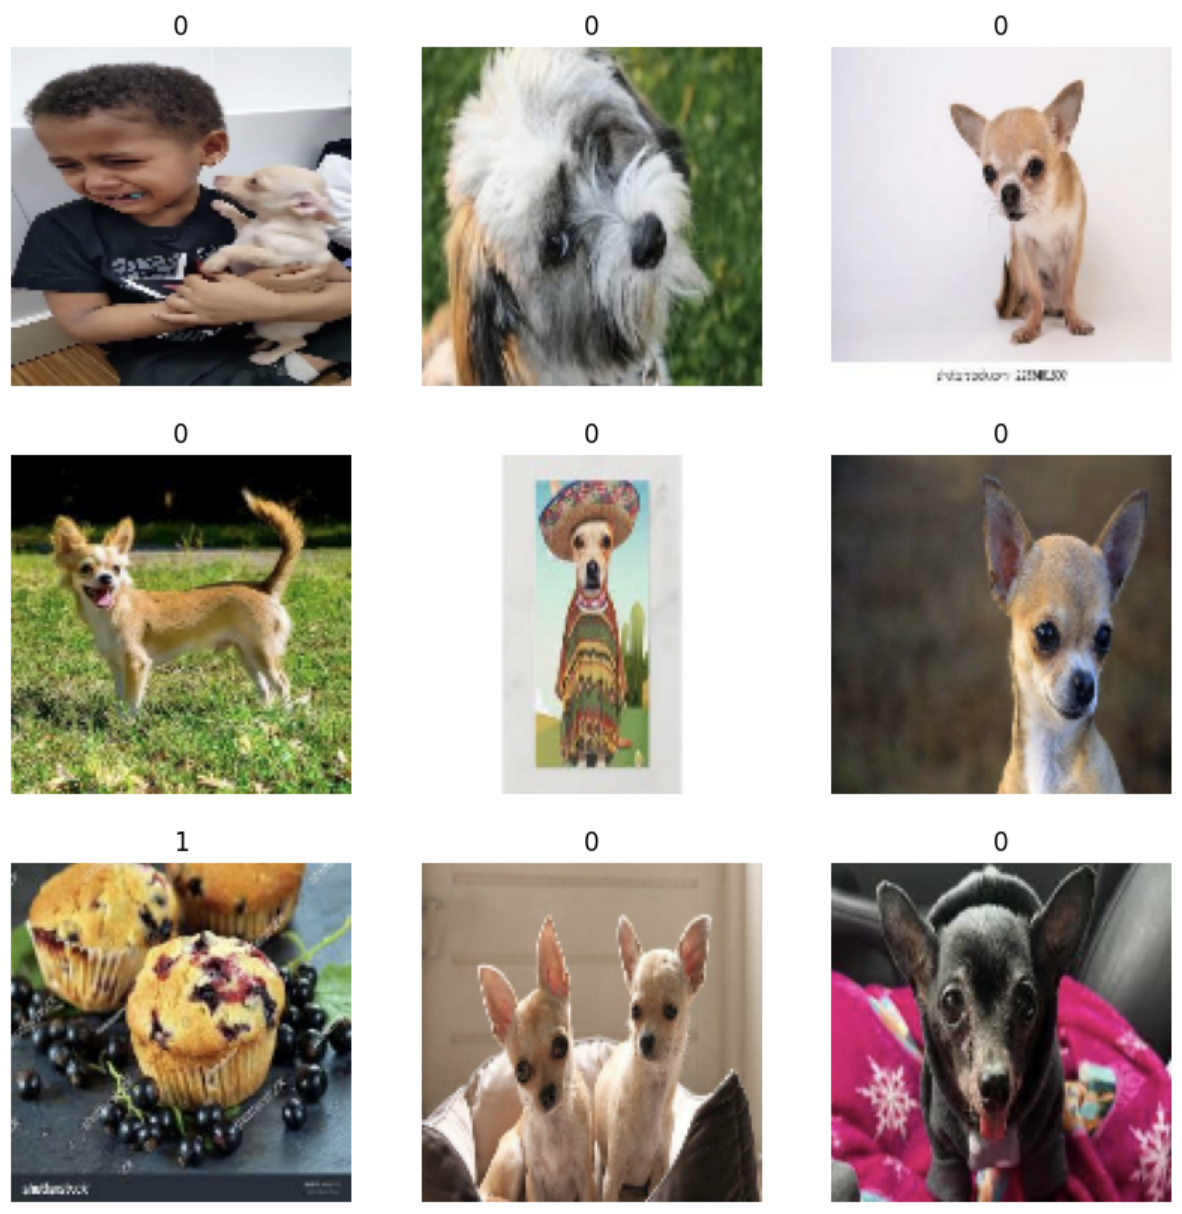
\includegraphics[scale=0.5]{../Images/sampleimages.png}
\end{figure}
As you can see muffin label is 0 and chihuahua label is 1.
\section{Preprocessing}
Certainly when dealing with data it is good to always make some improvement such as cleaning the data so that you have better results. In fact, the dataset was delivered without having duplicate images, which already represents a first step of preprocessing. In addition, I applied the \textbf{Data augmentation} \cite{dataaug} that is a technique in machine learning used to reduce overfitting when training a machine learning model, by training models on several slightly-modified copies of existing data.
With the help of Keras, it is possible to achieve date augmentation in the following way:
\begin{lstlisting}[language=Python]
data_augmentation = keras.Sequential(
    [
        layers.RandomFlip("horizontal"),
        layers.RandomRotation(0.1),
    ]
)
\end{lstlisting}
Here is graphically what the transformation looks like:
\begin{figure}[hbtp]
\caption{Data augmentation applied in a specific image}
\centering
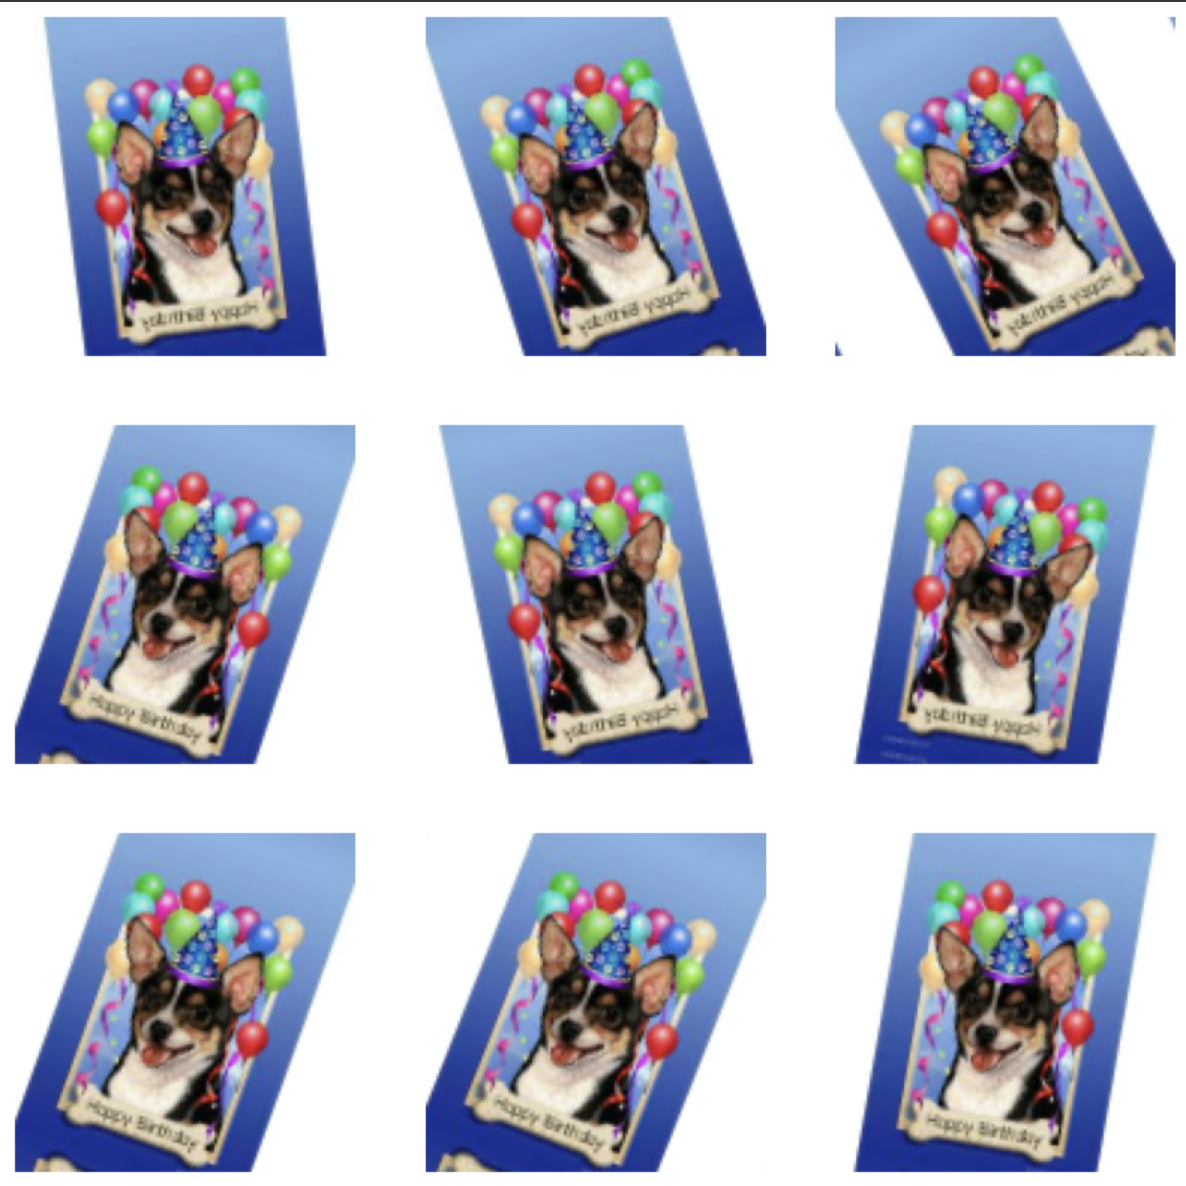
\includegraphics[scale=0.5]{../Images/dataaug.png}
\end{figure}
In order to complete the preprocessing I applied the data augmentation transformation to the input and I performed normalization of pixel values in the range [0, 255] to values in the range [0, 1], indeed this helps stabilize the training of the model. To conclude, this line 
\texttt{train\_images = train\_images.prefetch(tf.data.AUTOTUNE)} optimizes the data loading process during model training, allowing the model to work more efficiently and reducing the waiting time between data batches.




%
%			BIBLIOGRAFIA
%

\bibliographystyle{unsrt}
\bibliography{bibliografia}
\addcontentsline{toc}{chapter}{References}


\end{document}


 
